\chapter{Structural and accidental gaps\protect\symbolfootnote[1]{An abridged version of this chapter will appear in the proceedings of the 30th West Coast Conference on Formal Linguistics under the same name.}}
\label{clusters}

The term \emph{lexicon} has many senses: throughout, I use it to refer simply to the set of underlying representations.
%\citep[][269]{LANGUAGE}.

In the preceding chapter, it was proposed that 

Reconsider the null hypothesis presented in the preceding chapter:

\begin{example}[null hypothesis]
Universal grammar does not countenance constraints on the contents of URs
\end{example}

The idea 

relationship to proposal

One primary way which this null hypothesis has been critiqued is by demonstrating that the lexicon of some language 
exhibits dispreferences or gaps corresponding to.

argue by trends in the lexicon

possibility of sparsity (C\&H, Fischer/Vogt and recent stats)

Of course, to obtain the desired results, we must guarantee that each sequence structure rule reflects a general systematic fact about the language, and not a fact which is due merely to the existence of accidental gaps in the lexicon. \citep[][401, fn.~8]{Stanley1967}

In the preceding chapter, it was proposed that 

Lexicon

This appears to be exceptionlessly true of Arabic

That even gradient patterns 

One of the first study of this type was an analysis of co-occurrence restrictions on consonants in Javanese roots by \citet{Mester1988}, recently revisited by \citet{Graff2011}. 
Another Austronesian language studied in this fashion is Muna \citep{Coetzee2008a,Anttila2008}.
This technique has been applied to consonants in Semitic, especially Arabic \citep{McCarthy1988,McCarthy1994,Pierrehumbert1993,Frisch1996,Frisch2004,Coetzee2008a} but also in Tigrinya \citep{Buckley1997}, Hebrew \citep{Berent2003}, and Amharic \citep{Colavin2010}, and to various co-occurrence restrictions in English \citep{Berkley1994b,Berkley1994a,Pierrehumbert1994,Dmitrieva2008a,Dmitrieva2008b,Coetzee2008b}, Russian \citep{Padgett1992}, Dutch \citep{Graff2011}, Navajo \citep{Martin2007,Martin2011} and Gitksan \citep{Brown2010}.

The absence of 
The claim here is that however stark the absence or underrepresentation of some form is, it 

This hypothesis admits the possibility that there may be accidental gaps in the lexicon, a possibility which predates generative thinking:

\begin{quote}
\ldots{}the fact that some [clusters--KG] are not found must be due to accidental gaps in the inventory of signs, and cannot be explained by structural laws of the language. \citep[][16]{Fischer-Jorgensen1952}
\end{quote}

\noindent
Hans \citeauthor{Vogt1954} makes a similar observation in his study of Georgian clusters

\begin{quote}
Although my material is drawn from a fairly extensive corpus---all accessible dictionaries and vocabularies, printed texts of tens of thousands of pages as well as ordinary speech---there is every reason to believe, as experience has shown, that additional material would yield new clusters. The material will never be complete. It will always contain accidental gaps \ldots partly because some clusters by pure chance do not occur in the vocabulary. \citep[][30]{Vogt1954}
\end{quote}

\citet{Chomsky1965}

This chaper demonstrates that apparently systematic gaps may arise even in the absence of phonotactic preferences, and that this possibility compromises attempts to show that such preferences shape the lexicon. 

\section{Domain}

% WHY I'm DOING THIS STUDY
% describes makeup of the corpus and how p

\subsection{Data sources}

The English CELEX database \citep{CELEX},

\citet{Aronoff1976}

\citet{Harley2009}

\citet{Taft1975} ?
\citet{Taft1981} ?
\citet{Taft2004a} ?

\citet{Halle1962}

% 2.1.4: k

\subsubsection{Corpus counts}

Under the phonological analyses described in the next two sections, the 6,876 simplex words in CELEX contain 21 unique medial codas and 40 unique medial onsets. Of these 840 ($= 21 \times 40$) possible syllable contact clusters that could be produced by free combinations of the attested medials codas and onsets, 158 are attested, for a 18.8\% saturation rate.

\subsection{Syllabification}

For this task, it is necessary to separate medial consonant clusters into codas and onsets. While CELEX provides syllabified transcriptions, no description of the syllabification procedure is given in the documentation, and inspection of these syllabifications suggests the procedure used is not fully systematic. For instance, \emph{chemistry} is syllabified as [ˈkɛ.mɪ.strɪ] but \emph{ministry} as [ˈmɪ.nɪs.trɪ].\footnote{Note that word-final \emph{y} is generally lax [ɪ] in Received Pronunciation \citep[][294]{AOE2}.} This putative [ɪ.strɪ $\sim$ ɪs.trɪ] contrast, and many other such contrasts in the CELEX data, are dubious simply because there is no clear evidence that contrastive syllabification occurs in any language. Apparent counterexamples appear to be effects of vowel or consonant length \citep[e.g.,][]{Elfner2006}, word stress, or morphological structure, none of which explain the \emph{chemistry}/\emph{ministry} syllabification contrast.

An automated syllabification system was constructed and applied to medial clusters in the CELEX data. This system need only deal with simplex English words that contain the medial consonant clusters which are the focus of this study.  There is, for instance, no need to address the status of ``ambisyllabic'' consonants, i.e., singleton medial consonants preceded by a stressed lax vowel \citep[][219f.]{Rubach1996}, or to address morphological effects on syllabification. The technique used is a variation on the theme of onset maximization (e.g., \citealt{Kurylowicz1948}, \citealt[42f.]{Kahn1976}, \citealt[][?]{Selkirk1983}) which parses word-medial clusters so that the onset is as large as possible. Medial clusters in words like \emph{neu}[.tr]\emph{on} or \emph{bi}[.str]\emph{o} are found in word-initial position (e.g., [tr]\emph{ansit}, [str]\emph{ike}), and onset maximization leaves the coda of the first syllable empty. In contrast, the [nstr] cluster in \emph{mi}[n.str]\emph{el} does not occur word-initially; here the maximal onset is [str], and the [n] is assigned to the coda.

There is one case where unchecked maximization of medial onsets produces incorrect syllabifications. When a medial consonant cluster is preceded by a stressed lax vowel, as in words like \emph{propaga}[n.d]\emph{a}, \emph{whi}[s.p]\emph{er}, \emph{vi}[s.t]\emph{a}, or \emph{bi}[s.k]\emph{uit}, the first consonant of the cluster checks the lax vowel \citep[e.g.,][3]{Hammond1997}. \citet[][55]{Harris1994} notes that onset maximization makes the wrong predictions when the medial cluster is a valid onset: in \emph{whisper}, \emph{vista}, and \emph{biscuit}, it incorrectly assigns [sp, st, sk] to the medial onset, leaving the coda empty. The approach adopted here is to first apply onset maximization, then to reassign the first consonant of a medial onset to the preceding coda if it is immediately preceded by a stressed lax vowel.\footnote{\citet[][589f.]{Lowenstamm1981} observes a strikingly similar issue with the onset maximization principle in French, and proposes a similar solution.}

If the English affricates [tʃ, dʒ] are treated as sequences and not individual segments, this addition to the standard onset maximization technique would itself make the wrong prediction for medial affricates preceded by lax stressed vowels in words like \emph{ra}[.tʃ]\emph{et} or \emph{a}[.dʒ]\emph{ile}, incorrectly assigning the stop and fricative portions to separate syllables. For this reason, an additional constraint is assumed which prevents the two components of the affricates from being split by syllabification. This is motivated by the tendency of affricates to pattern with single segments in many languages. For instance, the only complex onsets in Classical Nahua are the affricates [ts, tʃ, tɬ] \citep[][9]{Launey2011}.

%In fact, [t.ʃ, d.ʒ] clusters are not found in simplex English words, despite the fact that that affricates occur as medial onsets in clusters (e.g., \emph{tru}[n.tʃ]\emph{eon}, \emph{so}[l.dʒ]\emph{er}).

\subsection{Inventory considerations}

To identify the inventory of syllable contact clusters, it is also necessary to parse syllables into onset, nucleus, and coda. In most cases this is trivial, but a few distributional heuristics for difficult cases are described below.

\subsubsection{The velar nasal}
\label{velarnasal}

There is a long-standing debate regarding whether English [ŋ] is a phoneme in its own right, as demanded by Kiparsky's Alternation Condition \citep{Kiparsky1968} or Lexicon Optimization \citep[][53]{OT}, or simply the allophone of /n/ found before /k, g/ \citep[][65]{Borowsky1986}. The strongest piece of evidence for treating the velar nasal as a pure allophone is the general absence of ?
nset [ŋ], a position where it can never be followed by a dorsal consonant needed to derive the velar allophone. \citet{Pierrehumbert1994} assumes the pure allophonic analysis in her study of syllable contact clusters, and it is assumed here. English nasal place allophony is formalized in Section \ref{cnpasection} below.
%\citealt[][62]{Halle1985a}),

\subsubsection{[j] onglides}

The [j] onglide in words such as in words such as \emph{ass}[j]\emph{ume} is assumed to be present in underlying representations (e.g., \citealt[][278]{Borowsky1986}, J. \citealt{Anderson1988b}, pace \emph{SPE}:196, \citealt[][89]{Halle1985a}, \citealt[][217]{McMahon1990}), since the presence or absence of the glide is at least marginally contrastive (e.g., \emph{coo}/\emph{coup} \alt{} \emph{queue}, \emph{booty} \alt{} \emph{beauty}). The front onglide is further assumed to be assigned to the nucleus, except when the onset would otherwise be null (e.g., \emph{jun}[j]\emph{or}). 
%\footnote{English glides are transcribed here as full segments, not as ``subsegments'', as this distinction does not appear to be meaningful for English, or empirically motivated for other languages \citep{Rubach2002}.}
There is extensive motivation for this principle. When [j] is a simplex onset, it may be followed by any vowel \citep[][276]{Borowsky1986}, but when [j] is immediately preceded by an onset consonant (e.g., [bj]\emph{ugle}), the following vowel is always [uː]. In fact, speakers judge words in which the front onglide is preceded by an onset consonant and followed by a vowel other than [uː] to be anomalous \citep{Moreland2009}. This defective distribution of vowels following [j] suggests that the onglide in this context is the first component of a phonological diphthong (\citealp[][232]{Hayes1980}, \citealp[][61f.]{Harris1994}, \citealp{Davis1995}). \citet[][42]{Clements1983} note that /m, v/ do not appear in onset clusters except in words like \emph{muse} or \emph{view}; the exceptionality of [juː] also suggests the glide is nuclear. There is also strong external support for this principle. The [juː] in words like \emph{spew} may pattern together in Pig Latin \citep{Davis1995,Idsardi2005} and \emph{shm}-reduplication \citep{Nevins2003} to the exclusion of the rest of preceding tautosyllabic consonants. The same fusion of [juː] at the expense of the onset is also found in speech errors, e.g., [kjuː]\emph{mor} [h]\emph{omponent} for [hjuː]\emph{mor component} \citep[][130]{Shattuck-Hufnagel1986}. Finally, \citet{Buchwald2005} considers [j] onglides in the speech of VBR, an aphasic patient who has difficulties producing complex onsets. 

\begin{example}[VBR's complex onsets (\citealp{Buchwald2005}:79--80, his transcriptions)] \label{VBR}
\begin{tabular}{l l l}
a. & kəræb  & `crab'  \\
   & bəlid  & `bleed' \\
b. & kəwin  & `queen' \\
   & kəwoʊt & `quote' \\
c. & kut    & `cute'  \\
   & musɪk  & `music  \\ 
\end{tabular}
\end{example}

\noindent
VBR breaks up complex onsets with epenthesis, including those that consist of a consonant and a back onglide cluster (\ref{VBR}b). However, no epenthesis occurs between a consonant and a front onglide; rather, the glide is absent (\ref{VBR}c). The failure of the front onglide to pattern with other consonant clusters suggests once again that the glide is part of the nucleus. 

%One potential problem with this account is noted by \citet{Kaye1996}, who obseres while [juː] may follow any single tautosyllabic consonant, it never follows branching onsets unless they consist of [s] and a single consonant. 
%This is the only sign that [juː] shows an affiliation for the onset. 

\subsubsection{[w] onglides}

The selective properties of the back onglide [w] contrast sharply with those of the front onglide, and I assume that it is assigned to the onset. Whereas the front onglide shows only limited selectivity for preceding tautosyllabic consonants \citep{Davis1995,Kaye1996}, the back onglide [w] is rarely preceded by tautosyllabic consonants other than [k] (e.g., \emph{tran}[kw]\emph{il}). Unlike the front glide, syllable-initial [kw] may be followed by nearly any vowel \citep[][161]{Davis1995}. Unlike [juː], onglide [w] followed by a vowel does not pattern together in Pig Latin \citep[][166]{Davis1995}. And onsets followed by [w] pattern with other complex onsets in undergoing epenthesis in the patholical speech of VBR, discussed immediately above.

%Whereas [Cjuː] syllables attracts stress, [kwV] syllables do not \citep[][162f.]{Davis1995}.

\subsubsection{Post-vocalic \emph{r}}

Both CELEX and the dictionary used by \citet{Pierrehumbert1994} in her study transcribe Received Pronunciation, in which word-medial post-vocalic \emph{r} has been lost. In \emph{r}-full dialects, there is reason to believe that post-vocalic \emph{r} is in fact nuclear, and therefore its presence or absence is irrelevant to the constraints on syllable contact clusters. Many vowel contrasts are suspended before \emph{r} \citep[][255]{Harris1994}; for example, \emph{fern}, \emph{fir}, and \emph{fur} lack the contrasts found in \emph{pet}, \emph{pit}, and \emph{putt}. Further evidence for the nuclear status of post-vocalic \emph{r} comes from variable phonological processes in which post-vocalic \emph{r} patterns differently than internal coda consonants. \citeauthor{Harris1994} reports that a variable process of /t/-\textsc{Glottalization} in many dialects of British English is blocked when /t/ is preceded by any consonant except post-vocalic \emph{r}.

\begin{example}[/t/-\textsc{Glottalization} in British English (after \citealp{Harris1994}:195, 258)]
\begin{tabular}{l l l@{} l}
a. & fis[t]   & * & fis[ʔ]   \\
   & mis[t]er & * & mis[ʔ]er \\
b. & par[t]   &   & par[ʔ]   \\
   & car[t]on &   & car[ʔ]on \\
\end{tabular}
\end{example}

\noindent Similarly, while /t, d/ delete in word-final position when immediately preceded by a consonant, including sonorants /n, l/, as in (\ref{td}a), deletion of /t, d/ after post-vocalic \emph{r} in American English is ``rare or nonexistent'' \citep[][8]{Guy1980}. 

\begin{example}[/t, d/-\textsc{Deletion}in American English] \label{td}
\begin{tabular}{l l l@{} l}
a. & be[lt]  &   & be[l]  \\
   & me[nd]  &   & me[n]  \\
b. & sh[ɚt]  & * & sh[ɚ] \\
   & c[ɚd]   & * & c[ɚ]  \\
\end{tabular}
\end{example}

%Finally, \citet[][251]{Fromkin1973} also presents evidence that post-vocalic \emph{r} may behave as if nuclear in speech errors. 

\section{Evaluation}

% what is being evaluated
% summary

\subsection{Static and derived constraints}

With this database of English syllable contact clusters it is now possible to evaluate constraints on sequences of underlying phonemes. 


Here, the metric used is simply 

The evaluation 

The foremost evidence for 


The evaluation used here is simply 

Having described the database of English syllable contact clusters, 



I now consider constraints on sequences of URs as predictors of attested and unattested contact clusters. First, I describe the statistical technique used, then apply this technique to both phonologically derived constraints and a set of ``static'' phonotactic constraints proposed by \citet{Pierrehumbert1994}. 

\subsubsection{Statistical technique}
\label{stattech}

Before the dawn of generative phonology, many linguists concerned themselves with documenting co-occurrence in various languages. \citet[][28]{Vogt1954} declares that a ``phonemic description of a language \ldots should also comprise a description of the phoneme combinations that occur or may be expected to occur in the language''. Studies in this tradition include the discussions of consononantal co-occurrence in Arabic and Javanese by \citet{Greenberg1950} and \citet{Uhlenbeck1950}, respectively. \citeauthor{Uhlenbeck1950}, for instance, puts forth co-occurrence dispreferences, rather than exceptionless generalizations of the sort given by \citet{Greenberg1950}. 

\citet{McCarthy1988}

Years later, \citet{Mester1988} revisits \citeauthor{Uhlenbeck1950}'s study and proposes a statistical technique, based on the chi-square test, to distinguish between accidental and structural lexical dispreferences in the Javanese lexicon. 

\citeauthor{Mester1988}'s technique has been adopted by many subsequent studies (e.g., \citealt{Padgett1992,Padgett1995} on Russian; \citealt{Pierrehumbert1993}, \citealt{Frisch1996}, and \citealt{Frisch2004} on Arabic; \citealt{Berkley1994b,Berkley1994a,Berkley2000}, \citealt{Dmitrieva2008a}, \citealt{Dmitrieva2008b} on English). The null hypothesis $H_0$ is that some sequence occurs at no different a rate than the researcher expects, and the alternative hypothesis $H_1$ is that it is underrepresented. Given an observed frequency $O$ and also a frequency $E$ expected under the null hypothesis, the test is as follows.

\begin{example}[null hypothesis testing]
$\displaystyle \textrm{Reject } H_0 \textrm{ iff } \frac{(O E) ^ 2}{E} >
χ^2$
\end{example}

%\footnote{This is the one-tailed version of the test.}
  
In this study, I use the \citet{Fisher1934} exact test, which is isomorphic to this chi-square test. Compared to the chi-square test, the Fisher exact test $p$-value is somewhat more difficult to compute, but both are automated by modern statistical packages and can be computed rapidly. The major advantage of the Fisher test over the chi-square test is that it is appropriate for small samples or rare events, whereas the chi-square test depends on an approximation which is only exact in the limit (i.e., with a hypothetically infinite sample), and therefore is not appropriate for small samples \citep[see][]{Gorman2012a}.
%\citep[e.g.,][142]{Mester1988}.

On the other end of the spectrum, the Monte Carlo statistical procedure developed by \citet{Kessler2001} and applied to co-occurrence statistics by \citet{Martin2007,Martin2011} and \citet{Brown2010} does not scale to large samples. The Monte Carlo procedure is isomorphic to the one-tailed Fisher Exact test, and involves comparing observed co-occurrence counts to those produced by randomly generated samples.  This requires the researcher to generate random permutations, something which is particularly difficult for large samples, as I will explain; disinterested readers may wish to skip the following paragraph.

Any permutation of a sequence $L$ can be represented as a sequence $S$ of the same length, where the value of $S_i$ corresponds to the permuted position of $L_i$. Generating random permutations requires an unbiased method to generate all $N!$ of these lists with equal probability. Unfortunately, this is near impossible for $N$s of moderate size with current computational resources. Any pseudo-random number generator can be characterized by its ``period'', the number of pseduo-random numbers it can emit before repeating itself; this is also the upper limit for the number of random permutations that can be generated. The pseudo-random number generator used by both \citeauthor{Martin2011} and \citeauthor{Brown2010} has a period of approximately $2^{48}$, a number which turns out to be smaller than $17!$. For the large samples, sometimes in the thousands, used by these researchers, virtually all the possible permutations can never be generated by this method. As a consequence, the shuffling procedure is far from random and introducing the possibility that the statistical test is biased in unpredictable ways.

As an example of the Fisher exact test as it is applied here, consider some of the Javanese co-occurrence facts considered by \citet{Mester1988}. \citeauthor{Mester1988} is at pains to show that there is a gradient dispreference for first and second root consonants which share the same major place. However, perfectly identical first and second consonants are exempt. Since 


% APPLY THIS TO JAVANESE

\begin{example}[Javanese root co-occurrence] %(\citealp[][264]{Uhlenbeck1950}, \citealp[][139]{Mester1988})]
\begin{tabular}{l r r r r}
\toprule
           & attested & unattested & saturation & $p$-value \\
\midrule
conforming & 134      & 12         & 0.918      & \multirow{2}{*}{6.095\e{-06}} \\
violating  & 21       & 15         & 0.583 \\
\bottomrule
\end{tabular}
\end{example}

\noindent
It is evident that roots with identical labial stops are far more common than those in which the roots disagree in voicing. 

This data is input to a chi-square test, which reports that this highly skewed distribution is unlikely to be due to chance 

That this is highly unlikely to be due to chance is apparent both from the chi-square ($\chi^2 = 25.572$, two-tailed $p = 4.3$\e{-07}) and Fisher exaact tests ($p =  6.095$\e{-06}). 

I use two-tailed statistical tests throughout. 
Under a one-tailed test, the alternative hypothesis is underrepresentation, whereas a two-tailed test also allows the possibility that a class of clusters would be overrepresented, i.e., more frequent than predicted by the null hypothesis. As 

\citet{Pierrehumbert1994}

It must be stressed that under current assumptions, this is independent of whether predictable prosodic representations (particularly coda and onset identity) are part of the memorized underlying representation \citep[e.g.,][]{Vaux2003}.
It is an undeniable fact that URs need to be 
The derivative nature of 
\citet{Ito1989a,Noske1992}

least some researchers (i.e., \citealt{Mester1988}) 

 \citep[e.g.,]{Brown2010} have argued for phonotactic constraints giving rise to overrepresentation, so I admit this possibility here and use two-tailed tests throughout. 

%\footnote{For example, \citet{Martin2007} applies this technique to a list of 4,758 noun-noun compounds. The number of permutations of a list of this length can be estimated using Stirling's approximation.

%\ex $ \lim_{n \rightarrow \infty} n! = e ^ {n \ln{n} - n} = 2 ^ {\log_2{e} (n \ln{n} - n)} $ \xe

%\noindent
%$4,758!$ is approximately $2 ^ {51260}$. The author is unaware of any system that provides 51,260 bits of entropy; and some popular programming languages, such as ANSI C, provide as few as 15 bits.}

%%% START OF SERIOUSNESS

I will first consider three well-known English phonological alternations, showing that these give rise to constraints on the sequence structure of morphs. Simple autosegmental formalizations of these processes are provided, and the Fisher exact test is used to demonstrate their effect on the English lexicon.

\subsubsection{Obstruent Voice Assimilation}

English has a process of voice assimilation which is found in two inflectional suffixes. The suffix /-d/ forms regular pasts and denominal adjectives, and /-z/ forms regular noun plurals and genitives, and the 3sg. present active indicative verbs.\footnote{The URs /-d, -z/ are argued for by \citet[][282]{Hockett1958}, \citet[][210]{SPE}, \citet{Basboll1972}, \citet{Shibatani1972}, S. \citet[][]{Anderson1973a}, \citet[][102]{Pinker1988}, and \citet[][284f.]{Bakovic2005b}, and alternative views are presented by \citet[][210f.]{LANGUAGE}, \citet[][426]{Nida1948}, \citet{Luelsdorff1969}, \citet{Lightner1970}, \citet{Hoard1971}, \citet[]{Miner1975}, \citet{Zwicky1975}, \citet{Kiparsky1985}, and \citet[][135]{Borowsky1986}.}

\begin{example}
Voice assimilation in the past tense and noun plural:

\vspace{0.5\baselineskip}
\begin{tabular}{l l l l l l}
a. & nap & nap[t] \\
   & nab & nab[d] \\
b. & lap & lap[s] \\
   & lab & lab[z]  \\
\end{tabular}
\end{example}

\noindent
The voiced obstruent suffixes devoice when preceded by a voiceless obstruent.
This is formalized as a rule spreading the [\textsc{Voice}] specification rightward over adjacent obstruents.

\begin{example}
\textsc{Obstruent Voice Assimilation} (\emph{SPE}:178): 

\xymatrix@R=24pt@C=24pt{
\txt{[α \textsc{Voice}]}\ar@{-}[d]\ar@{..}[dr] & \\
\txt{C}\ar@{-}[d]             & \txt{C}\ar@{-}[d] \\
\txt{[$+$\textsc{Obstruent}]} & \txt{[$+$\textsc{Obstruent}]}\\
}
\end{example}

\noindent
This rules out the possibility of surface clusters of obstruents with differing  [\textsc{Voice}] specifications. While the data make it clear \textsc{Obstruent Voice Assimilation} applies in morphologically derived environments, it is not obvious that it applies to obstruent clusters in non-derived environments (e.g., obstruent clusters in the URs of morphs) as well. \citet{Pierrehumbert1994} does not mention voice assimilation in her study of gaps in English syllable contact clusters. \citet[][74f.]{Hammond1999a} notes the existence of words like \emph{a}[b.s]\emph{inth} and \emph{a}[s.b]\emph{estos}, which contain obstruent voice clusters disagreeing in [\textsc{Voice}], and takes this as evidence that obstruent voicing is restricted to derived environments.

Despite these exceptions, I propose that \textsc{Obstruent Voice Assimilation} plays a major role in shaping the English lexicon. Only English syllable contact clusters which contain two adjacent obstruents speak to the status of \textsc{Obstruent Voice Assimilation}; the remaining 160 possible clusters are ignored. A $2 \times 2$ contingency table is constructed by dividing the remaining possible clusters into those which agree on obstruent voicing and those which do not, and into those which are attested and those which are not.

\begin{example}[Lexical effects of \textsc{Obstruent Voice Assimilation}]
\vspace{0.5\baselineskip}
\begin{tabular}{l r r r r}
\toprule
           & attested & unattested & saturation & $p$-value \\
\midrule
conforming & 80 & 370 & 0.178 & \multirow{2}{*}{1.1\e{-11}}\\
violating  &  6 & 264 & 0.022 \\
\bottomrule
\end{tabular}
\end{example}

\noindent 
18\% of the possible clusters containing adjacent obstruents with the same [\textsc{Voice}] specification are found, whereas only 2\%  of those which disagree in [\textsc{Voice}], such as in \emph{a}[b.s]\emph{inth} and \emph{a}[s.b]\emph{estos}, CELEX also contains \emph{jo}[d.p]\emph{urs}, \emph{pi}[ntʃ.b]\emph{eck}, \emph{sa}[k.b]\emph{ut}, and \emph{ja}[k.d]\emph{aw}. As the $p$-value shows, the rarity of these disagreeing clusters is unlikely to be due to chance. 

I propose that this pattern should be attributed directly to \textsc{Obstruent Voice Assimilation} applying to non-derived environments, preventing learners from positing URs in which adjacent obstruents do not agree in voice. There is no duplication between constraints on sequence structure and surface forms if both are derived from the application of the phonological rule (\citealt[][401f.]{Stanley1967}, \citealt[][382]{SPE}). The handful of exceptions to this generalization can be marked with appropriate exception diacritics. Another possibility is suggested by recent psycholinguistic results. \citet{Mattys2001b} find that 9-month old infants are sensitive to the contrast between [vt], a cluster of obstruents disagreeing in [\textsc{Voice}] which is not found word-medially, and [ft], which conforms to the above generalization and is found medially (e.g. \emph{a}[f.t]\emph{er}). This ability to use phonotactic violations to segment continuous speech persists into adulthood \citep{McQueen1998}, suggesting that ``hetero-voiced'' obstruent clusters may be analyzed as semantically opaque compounds by native speakers (e.g., \emph{ja}[k\#d]\emph{aw}). 
%\footnote{An analogous account is the proposal that readjustment rules insert morphological boundaries for the purposes of assigning stress (\emph{SPE}:94).}

\subsubsection{Coda nasal place assimilation}
\label{cnpasection}

Above, it was assumed that the velar nasal is derived from underlying /n/. 
This analysis is not purely allophonic, as nasal place assimilation alternations target the final consonant of the \emph{im-}/\emph{in-} prefix. In (\ref{npa}ab), the prefix-final consonant takes on the same major place of articulation as the following obstruent, and in (\ref{npa}c), where the root is vowel-initial, the prefix-final consonant is realized as a default /n/.

\begin{example}
\label{npa}
Nasal place assimilation in Latinate prefixes:

\vspace{0.5\baselineskip}
\begin{tabular}{l l l l}
%a. & possible & i[m.p]ossible & & balance & i[m.b]alance \\
%b. & tangible & i[n.t]angible & & decent  & i[n.d]ecent  \\
%c. & elegant  & i[n.]elegant  & & ability & i[n.]ability \\
a. & possible & i[m.p]ossible \\
   & balance  & i[m.b]alance  \\
b. & tangible & i[n.t]angible \\
   & decent   & i[n.d]ecent   \\
c. & elegant  & i[n]elegant  \\
   & ability  & i[n]ability  \\
\end{tabular} 
\end{example}

\noindent
The shape of the prefix before other obstruents is somewhat more complex. 
%Before /f/, CELEX transcribes the nasal as either labial or alveolar, the latter being very rare in simplex words. 
%There are also additional complexities regarding the shape of the prefix when attached to /k, g/-initial roots. 
\citet[][62]{Halle1985a} and \citet[][90]{Borowsky1986} report that coda nasals assimilate to [ŋ] before dorsal consonants, but this assimilation is blocked by stress on the following syllable, citing contrasts like the one between \emph{í}[ŋ.k]\emph{ubate} and \emph{i}[n.k]\emph{lúde}. The prefix \emph{com-}/\emph{con-}, which patterns with \emph{im-}/\emph{in-} in showing assimilation (e.g., \emph{co}[m.b]\emph{ine}), participates in a similar contrast, between \emph{có}[ŋ.g]\emph{ress} and \emph{co}[n.g]\emph{réssional}. As \citeauthor{Borowsky1986} notes, stress does not block assimilation in simplex words (e.g., \emph{a}[ŋ.g]\emph{óra}), a fact which demonstrates the necessity of a partially morphological explanation for the blocking of assimliation in words like \emph{co}[n.g]\emph{réssional}. Regardless of these complexities, there is sufficient evidence to posit assimilation of the \textsc{Place} features of an obstruent to a preceding nasal consonant. 

\begin{example}
\textsc{Coda Nasal Place Assimilation} (\emph{SPE}:85):

\xymatrix@R=24pt@C=24pt{
                          & \txt{\textsc{Place}}\ar@{-}[d]\ar@{..}[dl] \\
\txt{C}\ar@{-}[d]         & \txt{C}\ar@{-}[d] \\
\txt{[$+$\textsc{Nasal}]} & \txt{[$+$\textsc{Obstruent}]} \\
}
\end{example}

\citet[][175]{Pierrehumbert1994} observes that in simplex English words, ``nasal-stop sequences agree in labiality''; presumably, this generalization is limited to [\textsc{Labial}] because \citeauthor{Pierrehumbert1994} also adopts the assumption that the velar nasal is derived from /n/. However, \citeauthor{Pierrehumbert1994} does not propose any connection between the alternation and the generalization that nasal consonants in URs tend to agree with the following consonant. While clusters like \emph{pi}[m.p]\emph{le}, \emph{sta}[n.z]\emph{a}, and \emph{mo}[ŋ.k]\emph{ey} are the norm, exceptions like \emph{pli}[m.s]\emph{oll}, \emph{da}[m.z]\emph{el}, \emph{scri}[m.ʃ]\emph{aw}, and \emph{ra}[m.k]\emph{in} are found.

In all, there are only 80 possible nasal-obstruent syllable contact clusters, the majority of which are attested. In addition, there are a small number of words which contain clusters like \emph{oi}[nt.m]\emph{ent}, in which a nasal-obstruent cluster are both parsed into a complex medial coda, but in this position, place agreement is exceptionless, and thus these clusters are ignored below.

\begin{example}[Lexical effects of \textsc{Coda Nasal Place Assimilation}]
\begin{tabular}{l r r r r}
\toprule
           & attested & unattested & saturation & $p$-value \\
\midrule
conforming & 41 & 11 & 0.788 & \multirow{2}{*}{2.6\e{-05}}\\
violating  & 8  & 20 & 0.286 \\
\bottomrule
\end{tabular}
\end{example}

\noindent Clusters which conform to this generalization are far more likely to be attested than those that violate it, and this is highly unlikely to be due to chance.

There is some evidence that even young infants show a preference for nonce words that conform to this generalization. %\citet{Jusczyk2003}
\citet{Davidson2004}, \citet{Mattys1999}, and \citet{Jusczyk2002} play nonce words containing nasal-obstruent clusters to 4.5, 9, and 10-month-old infants (respectively) acquiring English, All three studies find that infants prefer to listen to stimuli which conform to the above generalization (e.g., \emph{u}[m.b]\emph{o}) over those which do not (e.g., \emph{u}[n.b]\emph{o}). \citet{Wright1975} taught several nonce words to a group of adolescents, and asked them to repeat the words to each other in a game of ``Telephone''. In these nonse words, nasals do not agree in \textsc{Place} with the following obstruent in these nonsense words, and \citeauthor{Wright1975} observes that after a few rounds of the game, the nonce words had been adapted to conform to \textsc{Coda Nasal Place Assimilation}.

\begin{example}[Artificial language adaptations (\citealt{Wright1975}:394, his transcriptions)]
\begin{tabular}{l l l l l l}
a. & [gownp] & > & [gump] \\
b. & [ǰumg]  & > & [ǰúŋgə] \\
c. & [ðʌŋd]  & > & [tɔŋg] \\
\end{tabular}
\end{example}

\noindent If this game is akin to the process of loanword adaptation, it is possible that various extragrammatical pressures are at play \citep[e.g.,][]{Halle1998b,Dupoux1999,Ussishkin2003,Peperkamp2008}. Yet, the independent evidence for a phonological process of nasal place assimilation provides the most parsiminious account of the adaptations seen in \citeauthor{Wright1975}'s study. J. \citet{Myers1993} also shows that \textsc{Coda Nasal Place Assimilation} is fed by speech errors:

\begin{example}[Speech errors and \textsc{Coda Nasal Place Assimilation} (\citealp{Myers1993}:228)]
\begin{tabular}{l l l}
   & \emph{error}  & \emph{target} \\
a. & primps        & prints        \\
b. & rand orker    & rank order    \\
%  & [sprɪg]time for [hɪ̃ntlɘr] & springtime for Hitler \\
c. & po[ŋ]cutation & computation   \\
\end{tabular} 
\end{example}

%\citet{Hay2004a} demonstrates that [n.p, mθ] clusters, which are not found in English, are in fact rated better than many attested clusters.
%report that 10-month-old infants prefer to listen to nonsense words which conform to \textsc{Coda Nasal Place Assimilation} (e.g., \emph{u}[m.b]\emph{o}) compared to those which do not (e.g., \emph{u}[n.b]\emph{o}). 

\subsubsection{Degemination}

A final well-known alternation in English is the simplification of geminates derived by certain suffixes. For instance, the suffix \emph{-ly} rarely forms a geminate when attaching to root-final /l/, whether forming denominal adjectives (e.g., \emph{sme}[l]\emph{y}) or deadjectival adverbs (e.g., \emph{norma}[l]\emph{y}). A small class of English verbs take a /-t/ suffix in the past; as this suffix does not trigger the \textsc{Epenthesis} found in the regular past (e.g., \citealt{Bakovic2005b}, \citealt{Fruehwald2011}), \textsc{Degemination} applies.

\begin{example}[Degemination in /-t/ pasts (\citealp{Halle1985a}:105, \citealp{Myers1987}:492)]
\begin{tabular}{l l l l l}
a. & burn    & burn[t] \\
   & spill   & spil[t] \\
b. & ben[d]  & ben[t]  \\
   & buil[d] & buil[t] \\
\end{tabular}
\end{example}

More complicated cases of degemination are found in English prefix morphology and described in \emph{SPE} (p.~148, 219f.) and \citealt[][]{Borowsky1986} (p. 102f.), and are not reviewed here.

%\ex \textsc{Coda Nasal Place Assimilation} feeds \textsc{Degemination} \citep[][116]{Borowsky1986}: \\
%\begin{tabular}{l l l l}
%a. & mature    & i[m]ature    & (cf. \emph{i}[m.b]\emph{alance})   \\
%b. & numerable & i[n]umerable & (cf. \emph{i}[n.d]\emph{ependent}) \\
%\end{tabular}
%\xe

The rule deletes the first of two adjacent consonants agreeing in \textsc{Place} and manner features, and is formalized using quantification over features \citep{Reiss2003b}.
% cf. \citep{Berent2012}

\begin{example}[\textsc{Degemination} (\emph{SPE}:253)]
\xymatrix@R=24pt@C=24pt{
\textsc{C}_1       & \longrightarrow & \emptyset & / & A~\gap\gap~A & \textsc{C}_2 \\
}
Condition: $\forall F_i \in \{\textsc{Place}, \textsc{Sonorant}, \textsc{Nasal}, \textsc{Continuant}, \textsc{Lateral}\}$ . $(F_i)_1 = (F_i)_2$
\end{example}

\noindent I assume that geminates crossing a syllable boundary are ``false geminates'', meaning that they are adjacent similar segments rather than a single feature matrix linked to two timing slots. Under the alternative account in which the absence of geminates is an inventory restriction (i.e., a \textsc{Segment Structure Condition}), an undesirable duplication of phonological derived surface constraints and constraints on URs would be unavoidable.

Neither identical consonants, nor those which differ only in voice (e.g., *[p.b]) occurs in simplex words in CELEX, and this absence is highly unlikely to be due to chance.

\begin{example}[Lexical effects of \textsc{Degemination}] 
\begin{tabular}{l r r r r}
\toprule
           & attested & unattested & saturation & $p$-value                   \\
\midrule
conforming & 157      & 596        & 0.208      & \multirow{2}{*}{7.2\e{-09}} \\
violating  & 0        &  87        & 0.000                                    \\
\bottomrule
\end{tabular}
\end{example}

%\footnote{Note that it is not the case that the English lexicon as envisioned by \emph{SPE} is free of underlying geminates; \citeauthor{SPE} use underlying geminates to attract stress to a preceding nucleus (p.~148--151). In \emph{SPE}, the underlying geminate-singleton contrast is absolutely neutralized, but has consequences for surface stress. In addition to the usual objections to absolute neutralization (i.e., that it is a learning conundrum mascarading as a phonological solution) that emerged in the wake of the publication of \emph{SPE}, the phonological particulars of this account have also come under attack \citep[e.g.,][]{Ross1972a}. It would not seem tenable to use underlying geminates to attract stress even if absolutely neutralized contrasts were admitted.} Unsurprisingly, this is unlikely to be due to chance. 

\subsubsection{Dorsal/non-coronal clusters}

\citet{Pierrehumbert1994} surveys the English syllable contact cluster inventory, and discerns the effect of several ``static'' constraints, those which do not derive from neutralizing phonological rules. 

\citet[][173]{Pierrehumbert1994} writes that ``velar obstruents occurred only before coronals in the clusters studied, never before labials or other velars.'' Since \citeauthor{Pierrehumbert1994}'s study is restricted to triconsonantal clusters, so words like \emph{a}[k.m]\emph{e}, \emph{ru}[g.b]\emph{y}, or \emph{pi}[g.m]\emph{ent} do not violate this narrower generalization. Further, \citeauthor{Pierrehumbert1994} adopts the traditional assumption \citep[e.g.,][66f.]{Borowsky1986} that coda [ŋ] is an allophone of /n/ before dorsal consonants, so words such as \emph{mo}[ŋ.gr]\emph{el} are not exceptions. 

\citeauthor{Pierrehumbert1994} generalization is termed static simply because there is no evidence for any phonological process which changes clusters of dorsal obstruents followed by non-coronals into something else (perhaps a dorsal/coronal cluster). However, the statistical test, taking into account clusters of any length, does not indicate that this dispreference for dorsal/non-coronal clusters is so compelling that it could not be generated by chance, simply because possible dorsal/non-coronal clusters are about as likely to occur as are similar types of clusters such as those with a non-dorsal coda and a non-coronal onset (e.g., \emph{a}[t.m]\emph{osphere}) or a dorsal coda and coronal onset (e.g., \emph{ve}[k.t]\emph{or}). These clusters are marked as ``conforming'' to a constraint \textsc{*[+Dorsal][$-$Coronal]}, and dorsal/non-coronal consonants as ``violating'' it. 

\begin{example}[Lexical effects of \textsc{*[$+$Dorsal][$-$Coronal]}]
\begin{tabular}{l r r r r}
\toprule
           & attested & unattested & saturation & $p$-value \\
\midrule
conforming & 76 & 359 & 0.175 & \multirow{2}{*}{0.145} \\
violating  &  6 &  57 & 0.095 \\
\bottomrule
\end{tabular}
\end{example}

There is no exceptions to \citeauthor{Pierrehumbert1994}'s narrower generalization concerning triconsonantal clusters, but it is no more statistically convincing. 

\begin{example}[Lexical effects of \textsc{*[$+$Dorsal][$-$Coronal]}, triconsonantal clusters only]
\begin{tabular}{l r r r r}
\toprule
           & attested & unattested & saturation & $p$-value              \\
\midrule
conforming & 20       & 148        & 0.119      & \multirow{2}{*}{0.136} \\
violating  &  0       &  22        & 0.000                               \\
\bottomrule
\end{tabular}
\end{example}

\noindent The evidence for \citeauthor{Pierrehumbert1994}'s static constraint does not actually require that such a constraint exists at all, since it is quite possible that the apparent dispreference for dorsal/non-coronal clusters could result by accident.

\subsubsection{Coda coronal obstruents}

Another static generalization about triconsonantal syllable contact clusters proposed by \citet[][175]{Pierrehumbert1994} is that  ``clusters with a coronal obstruent in the coda do not occur.'' In an endnote (p. 186), \citet{Pierrehumbert1994} notes an exception in \emph{a}[nt.l]\emph{er}, and one can add the triconsonantal clusters in \emph{ke}[s.tr]\emph{el} and \emph{oi}[nt.m]\emph{ent}, as well as many biconsonantal clusters like \emph{a}[t.l\emph{as} or \emph{e}[s.t]\emph{er}. As before, applying the statistical test to clusters of any length reveals that coda coronal obstruent clusters are not significantly less likely to occur than clusters with non-coronal codas. 

\begin{example}[Lexical effects of \textsc{*Coda Coronal Obstruent}]
\begin{tabular}{l r r r r}
\toprule
           & attested & unattested & saturation & $p$-value              \\
\midrule
conforming & 48       & 312        & 0.133      & \multirow{2}{*}{0.301} \\
violating  & 38       & 322        & 0.106                               \\
\bottomrule
\end{tabular}
\end{example}

Restricting \citeauthor{Pierrehumbert1994}'s generalization to triconsonantal clusters does not strengthen the case for this static constraint.

% there isn't really any theoretical argument for triconsonantal clusters only 

\begin{example}[Lexical effects of \textsc{*Coda Coronal Obstruent}, triconsonantal clusters only]
\begin{tabular}{l r r r r}
\toprule
           & attested & unattested & saturation & $p$-value \\
\midrule
conforming & 4        & 104        & 0.037      & \multirow{2}{*}{0.419} \\
violating  & 2        & 124        & 0.016                               \\
\bottomrule
\end{tabular} 
\end{example}

%Note that [tʃ] has not been included since it so rarely occurs in clusters.

\subsubsection{ABA clusters}

Finally, \citet[][176]{Pierrehumbert1994} notes ``a lack of clusters with identical first and third elements''. For the determination of identity, I assume the same definition of geminate as used in the rule of \textsc{Degemination} above, namely consonants which share all the same \textsc{Place} and manner features, ignoring \textsc{Voice}. 
%and I also expand the definition of the constraint to also apply to the second and fourth consonant of quadraconsonantal clusters. 
\citeauthor{Pierrehumbert1994} notes one potential exception to this generalization, the cluster in words such as \emph{e}[ks.kl]\emph{ude}, which contains two /k/, does not arise here since such words have been marked morphologically complex. Despite the fact that the corpus contains no exceptions to this generalization, these \textsc{ABA} clusters are not significantly rarer than other triconsonaontal and quadraconsonantal clusters, of which only 7.8\% occur. 

\begin{example}[Lexical effects of \textsc{*aba}]
\begin{tabular}{l r r r r}
\toprule
           & attested & unattested & saturation & $p$-value \\
\midrule
conforming & 41       & 478        & 0.079      & \multirow{2}{*}{0.818} \\
violating  &  0       &  11        & 0.000                               \\
\bottomrule
\end{tabular}
\end{example}

Whereas the three alternations targeting English syllable contact clusters have robust lexical reflexes as measured by the Fisher exact test, such tests reveal no evidence for the static dispreferences identified by \citeauthor{Pierrehumbert1994}.

%\subsubsection{Summary}
%
%The above results are summarized in Table \ref{constraints}.
%
%\begin{table}
%\centering
%\begin{tabular}{l r r r r r}
%\toprule
%                                       & \multicolumn{2}{c}{attested} & \multicolumn{2}{c}{unattested} & \multirow{2}{*}{$p$-value} \\
%                                       & conforming & violating & conforming & violating \\
%\midrule
%\textsc{O.V.A.} (\ref{ovar})        &  80 &   6 & 370 & 264 & 1.1\e{-11} \\
%\textsc{C.N.P.A} (\ref{CNPA})       &  41 &  25 &  12 &  42 & 1.7\e{-05} \\ 
%\textsc{Degemination} (\ref{degem}) & 161 & 632 &   0 &  87 & 1.4\e{-08} \\
%\midrule
%\textsc{*Dorsal-Labial} ()          &  68 &   4 & 246 &  40 & 0.069 \\
%\textsc{*C.C.O.} ()                 &  48 &  38 & 312 & 322 & 0.301 \\
%\textsc{*A,BA} ()                   & 161 &   0 & 708 &  11 & 0.231 \\
%\bottomrule
%\end{tabular}
%\caption{Counts and Fisher exact test $p$-values for the constraints discussed above.}
%\label{constraints}
%\end{table}

\subsection{Computational models}

Applying these derived constraints to the lexicon increases saturation from 18.8\% to 28.8\% and incurs only a handful of exceptions. Yet, despite the fact that ``attestation'' is the minority pattern, attempts to identify static lexical constraints, whether by hand or computational model, lend little additional predictive power. There is no evidence that the English syllable contact inventory is subject to any static constraint at all. I am forced to conclude that most, if not all, of 71.2\% of possible clusters which are unattested are accidental gaps. Below, I show that this state of affairs follows directly from the sparse distribution of codas and onsets. 

The three alternations targeting English syllable contact clusters have been shown to have the expected robust effects on the English lexicon. 


Whereas the three alternations targeting English syllable contact clusters have robust lexical reflexes as measured by the Fisher exact test, such tests reveal no evidence for the static dispreferences identified by \citeauthor{Pierrehumbert1994}. There is now a growing literature on computational cognitive models of phonotactic learning. By applying these models to the syllable contact data, it is possible to exhaustively search for statistically motivated constraints, elimianting the possibility of human error. 

To evaluate these statistical models, they are first trained on the set of attested clusters, then put to the task of classifying all possible clusters into those which are and are not attested. Four metrics are used to evaluate these computational models. Classification accuracy corresponds to the probability of a classification being either a true positive ($t.p.$), correctly predicting a cluster to occur, or a true negative ($t.n.$), correctly predicting a cluster to be absent. Incorrect outcomes are either false positives ($f.p.$), incorrectly predicting a cluster to occur, and false negatives ($f.n.$), incorrectly predicting a cluster to be absent. 

%Binary classification contingency table: \\
%\begin{tabular}{c | l l} \toprule
%                             & \multicolumn{2}{c}{prediction} \\
%\midrule
%\multirow{2}{*}{observation} & true positive ($tp$)  & false positive ($fp$) \\
%                             & false negative ($fn$) & true negative ($tn$) \\
%\end{tabular}
%\begin{tabular}{|l l|}
%\toprule
%true positive ($tp$)  & false positive ($fp$) \\
%false negative ($fn$) & true negative ($tn$) \\
%\bottomrule
%\end{tabular}

\begin{unlabeledexample}
$\displaystyle \textrm{Accuracy} = \frac{t.p. + t.n.}{t.p. + t.n. + f.p. + f.n.}$
\end{unlabeledexample}

\noindent A few other metrics can be used to assess classification performance. Precision corresponds to the probability that a cluster predicted to occur is observed in the data. 

\begin{unlabeledexample}
$\displaystyle \textrm{Precision} = \frac{t.p.}{t.p. + f.p.}$ 
\end{unlabeledexample}

\noindent Recall (also known as sensitivity) is the probability a observed cluster is predicted to occur. 

\begin{unlabeledexample}
$\displaystyle \textrm{Recall} = \frac{t.p.}{t.p. + f.n.}$
\end{unlabeledexample}

It is possible to maximize recall at the expense of precision, by predicting more clusters to be attested, or to increase precision at the expense of recall by predicting fewer clusters to be attested. A common way to balance these concerns is the $F_1$ score, which is the harmonic mean of precision and recall.

\begin{unlabeledexample}
$\displaystyle F_1 = 2 \left( \frac{\textrm{Precision} \times \textrm{Recall}}{\textrm{Precision} + \textrm{Recall}}\right)$ 
\end{unlabeledexample}

\subsubsection{Null baseline}

The 840 possible clusters have an 18.7\% of saturdaion rate. As a consequence of this sparsity, a null model which classifies all clusters as unattested achieves 81.3\% accuracy without the need to posit any constraints either derived or static. Since this model does not have any positive classifications, either true or false, precision, recall, and $F_1$ are undefined.

\subsubsection{Alternations}

As was shown above, \textsc{Obstruent Voice Assimiation}, \textsc{Coda Nasal Place Assimilation}, and \textsc{Degemination} are reliable predictors of what clusters are and are not attested and have few lexical exceptions. I generate another baseline by predicting only those clusters which do not violate any of these generalizations to be attested. This provides a significant improvement to the null baseline (accuracy = 0.857). As precision (0.401) is smaller than recall (0.708), there are more false positives (i.e., unattested clusters that do not violate any of these three alternation-derived generalizations) than there are false negatives (i.e., attested exceptions to these derived generalizations). 

\subsubsection{\citet{Pierrehumbert1994}}

\citet{Pierrehumbert1994} first proposes to measure the well-formedness of syllable contact clusters by the independent probabilities of codas and onsets, and \citet{Coleman1997} extend this model to whole words. \citet{Pierrehumbert1994} uses both medial and initial/final codas and onsets to compute these probabilities, but I obtain a better fit to the data by only using medial coda and onset frequencies. Medial coda and onset probabilities are multipled to obtain a well-formedness score. This produces a continuous value between 0 and 1. To derive a binary classification from these values, I use a soft-margin support vector machine \citep{Cortes1995} with a linear kernel. This technique derives a ``decision stump'' providing the best single split into attested and an unattested clusters. This is not put forth as a cognitively plausible model for relating this expected probability to attestation: it is simply the upper bound that such a model could reach. 

Unfortunately, this score only provides a small improvement to the null baseline
 (accuracy = 0.839), and has a lower accuracy and $F_1$ (0.328) than the alternation baseline. 

\subsubsection{\citet{Hayes2008a}}

\citeauthor{Hayes2008a} develop a sophisticated method of learning phonotactic distributions from positive data. They develop software for estimating probability distributions over sequences of (sets of) phonological features using the principle of maximum entropy and making few assumptions about the independence of features. As above, a support vector machine with a linear kernel is used to turn these probability values into binary predictions. The software provided by these authors exposes many ``metaparameters'', operational decisions to be made in conducting an experiment with this system. To avoid any potential bias induced by the choice of these metaparameters, I use the same settings as used by \citet{Hayes2008a} in their similar study of English onset consonants. This includes the ``accuracy schedule'' [0.001, 0.01, 0.1, 0.2, 0.3] and no constraints on the number of constraints learned, as well English consonantal features used by \citeauthor{Hayes2008a}. Since this model is inherently stochastic, producing slightly different outcomes on each run, I follow the practice of \citeauthor{Hayes2008a} (p.~396) and report the lowest-accuracy of ten runs, though in general there is not a great deal of variation between individual runs.  

This model provides a small improvement in accuracy (0.877) and $F_1$ (0.703) compared to the alternation baseline, but it has lower recall (0.642) than this baseline, indicating that the \citeauthor{Hayes2008a} model introduces many false negatives. 
%; it assigns the lowest probability value to 122 unattested clusters.
More specifically, it suggests that this model prefers narrower phonotactic generalizations than those derived from alternations. For instance, unattested *[m.kl] is assigned the highest probability, whereas it is ruled out by \textsc{Coda Nasal Place Assimilation}. On the other hand, the \citeauthor{Hayes2008a} model assigns a low score to clusters like those found in \emph{hu}[z.b]\emph{and} and \emph{pla}[t.f]\emph{orm}, though they are both attested and consistent with all three alternation-derived constraints. 

\citet{Berent2012} identify an important defect with the \citeauthor{Hayes2008a} model used here: it does not make use of variables over features and thus fails to unify the constraint against geminate clusters. While the model may miss this unifying generalization, it correctly predicts all clusters containing geminates to be unattested. 

The results for the four models are summarized below.

\begin{example}[Summary of computational models]
\begin{tabular}{l | r r r r}
\toprule
                          & accuracy & precision & recall & $F_1$ \\ 
\midrule
Null baseline             & 0.813    & n.a.      & n.a.   & n.a.  \\
Alternations              & 0.857    & 0.401     & 0.708  & 0.512 \\
\citet{Pierrehumbert1994} & 0.839    & 0.210     & 0.750  & 0.328 \\
\citet{Hayes2008a}        & 0.877    & 0.777     & 0.642  & 0.703 \\
\bottomrule
\end{tabular}
\end{example}

One additional model was evaluated for this study. \citet{McGowan2011} claims that the type frequency of individual syllable contact clusters in English is predicted by the change of sonority in the clusters.\footnote{Thanks to Maria Gouskova for bringing this study to my attention.} Using a sonority scale proposed by \citet{Jespersen1904}, \citeauthor{McGowan2011} reports that clusters like [m.p], with sharply falling sonority, are slightly more frequent than those like [t.j], with rising sonority. However, \citeauthor{McGowan2011} finds that sonority of clusters accounts for only a tiny amount of the variance in cluster frequency ($R^2 = 0.077$). In this study, inclusion of sonority distance provided no improvement over the null baseline, and therefore was not considered further.

\subsection{Computational models}

Applying these derived constraints to the lexicon increases saturation from 18.8\% to 28.8\% and incurs only a handful of exceptions. Yet, despite the fact that ``attestation'' is the minority pattern, attempts to identify static lexical constraints, whether by hand or computational model, lend little additional predictive power. There is no evidence that the English syllable contact inventory is subject to any static constraint at all. I am forced to conclude that most, if not all, of 71.2\% of possible clusters which are unattested are accidental gaps. Below, I show that this state of affairs follows directly from the sparse distribution of codas and onsets. 

The three alternations targeting English syllable contact clusters have been shown to have the expected robust effects on the English lexicon. 

Whereas the three alternations targeting English syllable contact clusters have robust lexical reflexes as measured by the Fisher exact test, such tests reveal no evidence for the static dispreferences identified by \citeauthor{Pierrehumbert1994}. There is now a growing literature on computational cognitive models of phonotactic learning. By applying these models to the syllable contact data, it is possible to exhaustively search for statistically motivated constraints, elimianting the possibility of human error. 

To evaluate these statistical models, they are first trained on the set of attested clusters, then put to the task of classifying all possible clusters into those which are and are not attested. Four metrics are used to evaluate these computational models. Classification accuracy corresponds to the probability of a classification being either a true positive ($t.p.$), correctly predicting a cluster to occur, or a true negative ($t.n.$), correctly predicting a cluster to be absent. Incorrect outcomes are either false positives ($f.p.$), incorrectly predicting a cluster to occur, and false negatives ($f.n.$), incorrectly predicting a cluster to be absent. 

%\ex Binary classification contingency table: \\
%\begin{tabular}{c | l l} \toprule
%                             & \multicolumn{2}{c}{prediction} \\
%\midrule
%\multirow{2}{*}{observation} & true positive ($tp$)  & false positive ($fp$) \\
%                             & false negative ($fn$) & true negative ($tn$) \\
%\end{tabular}
%\begin{tabular}{|l l|}
%\toprule
%true positive ($tp$)  & false positive ($fp$) \\
%false negative ($fn$) & true negative ($tn$) \\
%\bottomrule
%\end{tabular}
%\xe 

It is possible to maximize recall at the expense of precision, by predicting more clusters to be attested, or to increase precision at the expense of recall by predicting fewer clusters to be attested. A common way to balance these concerns is the $F_1$ score, which is the harmonic mean of precision and recall.

\subsubsection{Null baseline}

The 840 possible clusters have an 18.7\% of saturdaion rate. As a consequence of this sparsity, a null model which classifies all clusters as unattested achieves 81.3\% accuracy without the need to posit any constraints either derived or static. Since this model does not have any positive classifications, either true or false, precision, recall, and $F_1$ are undefined.

\subsubsection{Alternations}

As was shown above, \textsc{Obstruent Voice Assimiation}, \textsc{Coda Nasal Place Assimilation}, and \textsc{Degemination} are reliable predictors of what clusters are and are not attested and have few lexical exceptions. I generate another baseline by predicting only those clusters which do not violate any of these generalizations to be attested. This provides a significant improvement to the null baseline (accuracy = 0.857). As precision (0.401) is smaller than recall (0.708), there are more false positives (i.e., unattested clusters that do not violate any of these three alternation-derived generalizations) than there are false negatives (i.e., attested exceptions to these derived generalizations). 

\subsubsection{\citet{Pierrehumbert1994}}

\citet{Pierrehumbert1994} first proposes to measure the well-formedness of syllable contact clusters by the independent probabilities of codas and onsets, and \citet{Coleman1997} extend this model to whole words. \citet{Pierrehumbert1994} uses both medial and initial/final codas and onsets to compute these probabilities, but I obtain a better fit to the data by only using medial coda and onset frequencies. Medial coda and onset probabilities are multipled to obtain a well-formedness score. This produces a continuous value between 0 and 1. To derive a binary classification from these values, I use a soft-margin support vector machine \citep{Cortes1995} with a linear kernel. This technique derives a ``decision stump'' providing the best single split into attested and an unattested clusters. This is not put forth as a cognitively plausible model for relating this expected probability to attestation: it is simply the upper bound that such a model could reach. 

Unfortunately, this score only provides a small improvement to the null baseline
 (accuracy = 0.839), and has a lower accuracy and $F_1$ (0.328) than the alternation baseline. 

\subsubsection{\citet{Hayes2008a}}

\citeauthor{Hayes2008a} develop a sophisticated method of learning phonotactic distributions from positive data. They develop software for estimating probability distributions over sequences of (sets of) phonological features using the principle of maximum entropy and making few assumptions about the independence of features. As above, a support vector machine with a linear kernel is used to turn these probability values into binary predictions. The software provided by these authors exposes many ``metaparameters'', operational decisions to be made in conducting an experiment with this system. To avoid any potential bias induced by the choice of these metaparameters, I use the same settings as used by \citet{Hayes2008a} in their similar study of English onset consonants. This includes the ``accuracy schedule'' [0.001, 0.01, 0.1, 0.2, 0.3] and no constraints on the number of constraints learned, as well English consonantal features used by \citeauthor{Hayes2008a}. Since this model is inherently stochastic, producing slightly different outcomes on each run, I follow the practice of \citeauthor{Hayes2008a} (p.~396) and report the lowest-accuracy of ten runs, though in general there is not a great deal of variation between individual runs.  

This model provides a small improvement in accuracy (0.877) and $F_1$ (0.703) compared to the alternation baseline, but it has lower recall (0.642) than this baseline, indicating that the \citeauthor{Hayes2008a} model introduces many false negatives. 
%; it assigns the lowest probability value to 122 unattested clusters.
More specifically, it suggests that this model prefers narrower phonotactic generalizations than those derived from alternations. For instance, unattested *[m.kl] is assigned the highest probability, whereas it is ruled out by \textsc{Coda Nasal Place Assimilation}. On the other hand, the \citeauthor{Hayes2008a} model assigns a low score to clusters like those found in \emph{hu}[z.b]\emph{and} and \emph{pla}[t.f]\emph{orm}, though they are both attested and consistent with all three alternation-derived constraints. 

\citet{Berent2012} identify an important defect with the \citeauthor{Hayes2008a} model used here: it does not make use of variables over features and thus fails to unify the constraint against geminate clusters. While the model may miss this unifying generalization, it correctly predicts all clusters containing geminates to be unattested. 

The results for the four models are summarized below.

\begin{example}
Summary of computational model accuracy: 

\vspace{0.5\baselineskip} 
\begin{tabular}{l | r r r r}
\toprule
                          & accuracy & precision & recall & $F_1$ \\ 
\midrule
Null baseline             & 0.813    & n.a.      & n.a.   & n.a.  \\
Alternations              & 0.857    & 0.401     & 0.708  & 0.512 \\
\citet{Pierrehumbert1994} & 0.839    & 0.210     & 0.750  & 0.328 \\
\citet{Hayes2008a}        & 0.877    & 0.777     & 0.642  & 0.703 \\
\bottomrule
\end{tabular}
\end{example}

One additional model was evaluated for this study. \citet{McGowan2011} claims that the type frequency of individual syllable contact clusters in English is predicted by the change of sonority in the clusters.\footnote{Thanks to Maria Gouskova for bringing this study to my attention.} Using a sonority scale proposed by \citet{Jespersen1904}, \citeauthor{McGowan2011} reports that clusters like [m.p], with sharply falling sonority, are slightly more frequent than those like [t.j], with rising sonority. However, \citeauthor{McGowan2011} finds that sonority of clusters accounts for only a tiny amount of the variance in cluster frequency ($R^2 = 0.077$). In this study, inclusion of sonority distance provided no improvement over the null baseline, and therefore was not considered further.

\subsection{Statistical properties of syllable contact}

Constraints on 

Above, we have seen that constraints on URs which are derive from phonological alternations restrict the contents of the lexicon. 


Applying these derived constraints to the lexicon increases saturation from 18.8\% to 28.8\% and incurs only a handful of exceptions. Yet, despite the fact that ``attestation'' is the minority pattern, attempts to identify static lexical constraints, whether by hand or computational model, lend little additional predictive power. There is no evidence that the English syllable contact inventory is subject to any static constraint at all. I am forced to conclude that most, if not all, of 71.2\% of possible clusters which are unattested are accidental gaps. Below, I show that this state of affairs follows directly from the sparse distribution of codas and onsets. 

\subsubsection{The $Z_r$ transform}

In a sparse distribution, many types occur at the same low frequencies. \citet{Good1953} notes that this produces a type of quantization, an artificially long and flat right tail in the frequency spectrum. \citet[][29]{Church1991} propose a method to eliminate this quantization, the $Z_r$ transform, defined as follows.
Let $r, n$ be defined such that $n_i$ is the number of types which occur at frequency $r_i$ (i.e., $n$ contains frequencies of type frequencies). Further, let $r$ be sorted in increasing order. $Z$ is simply each element of $n$ scaled by the nearest points to the left and right. 

\begin{unlabeledexample}
$\displaystyle Z_i = \frac{2 n_i}{r_{i + 1} - r_{i - 1}}$
\end{unlabeledexample}

\noindent \citeauthor{Church1991} do not define this transform for the lowest and highest points (i.e., when $i = 1$ or $i = N$), and so I extend the definition by scaling these points using only one inward-facing point.

\begin{unlabeledexample}
$\displaystyle Z_1 = \frac{n_1}{r_2 - r_1}$
\end{unlabeledexample}

\begin{unlabeledexample}
$\displaystyle Z_N = \frac{n_N}{r_N - r_{N - 1}}$
\end{unlabeledexample}

%\indent
%The effect of this transform can be seen in Figure \ref{zr}. 

%\begin{figure}
%\centering
%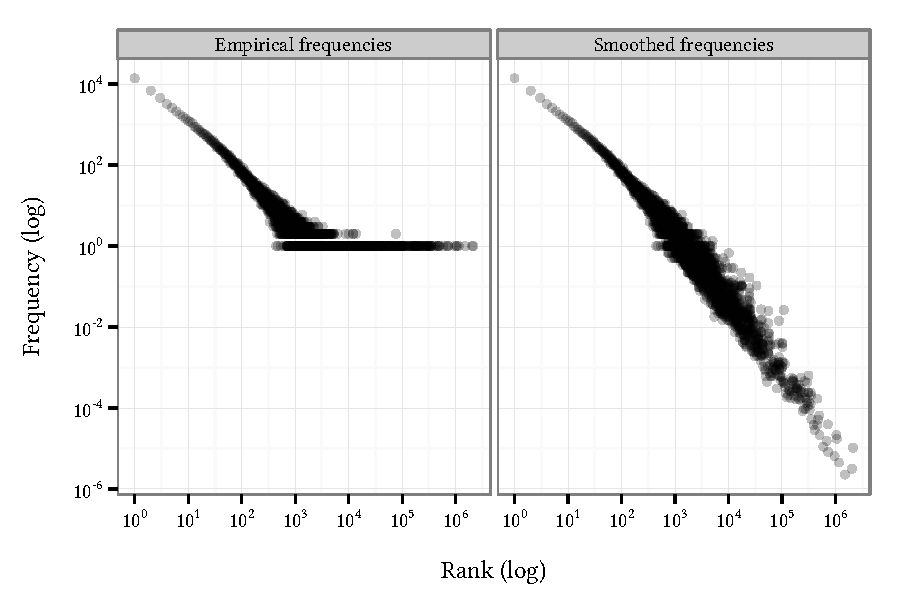
\includegraphics{zr.pdf}
%\caption{The SUBTLEX word frequency norms \citep{Brysbaert2009} show a long right tail in the log-frequency/log-rank space (left panel), and the $Z_r$ transform (right panel) smooths out this tail.}
%\label{zr}
%\end{figure}

\subsubsection{Coda, onset, and cluster sparsity}

A number of previous studies \citep[e.g.,][]{Sigurd1968,Good1969,Borodovsky1989,Witten1990,Martindale1996,Tambovtsev2007} have observed that phonemes and graphemes exhibit sparse type (i.e., lexical) and token frequency distributions. The lexical frequencies of the medial codas ond onsets which make up syllable contact clusters show a similar distribution. In Figure \ref{codaonset}, $Z_r$-transformed lexical frequencies of codas and onsets are plot against rank, in log-log spaces. The near-linear relationship that obtains indicates that the data can be modeled by a generalization of Zipf's law \citep{Zipf1949}.

%\begin{figure}
%\centering
%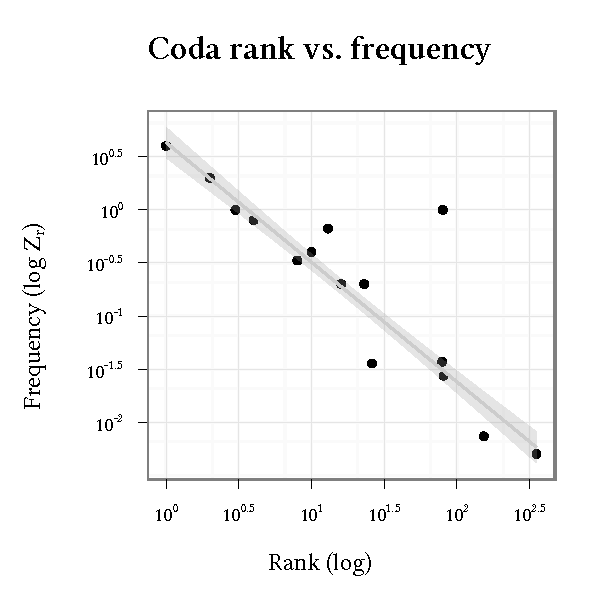
\includegraphics{coda.pdf} 
%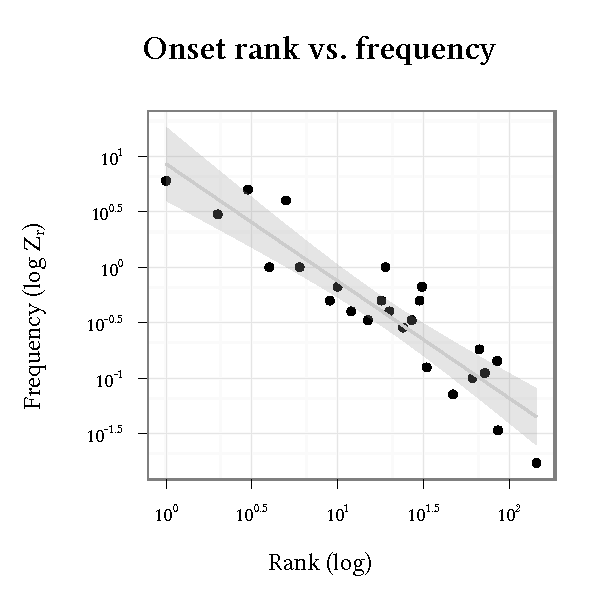
\includegraphics{onset.pdf}
%\caption{Medial coda and medial onset lexical frequency exhibit the Zipfian log-log-linear relationship between rank and frequency.}
%\label{codaonset}
%\end{figure}

\begin{unlabeledexample}
$\displaystyle f(r; C, \alpha) = \frac{C}{r^\alpha}$ 
\end{unlabeledexample}

\noindent The parameters $C$, a constant sensitive to sample size, and $\alpha$, the slope of the rank/frequency relationship in log-log space, are easily computed using the method of least squares in a linear regression, where $\epsilon$ represents the error term.

\begin{example}[example]
$\displaystyle \textrm{log}~Z_r \sim C + \alpha~\textrm{log}~r + \epsilon$ 
\end{example}

\noindent Codas ($\alpha = -0.720$, $R^2 = 0.749$) and onsets ($\alpha = -1.056$, $R^2 = 0.828$) are well-fit by this distribution, though there are some outliers. Similarly, clusters, shown in Figure \ref{clus}, are also a good fit to the generalized Zipf's law ($\alpha = -0.588$, $R^2 = 0.924$). 

\begin{figure}
\centering
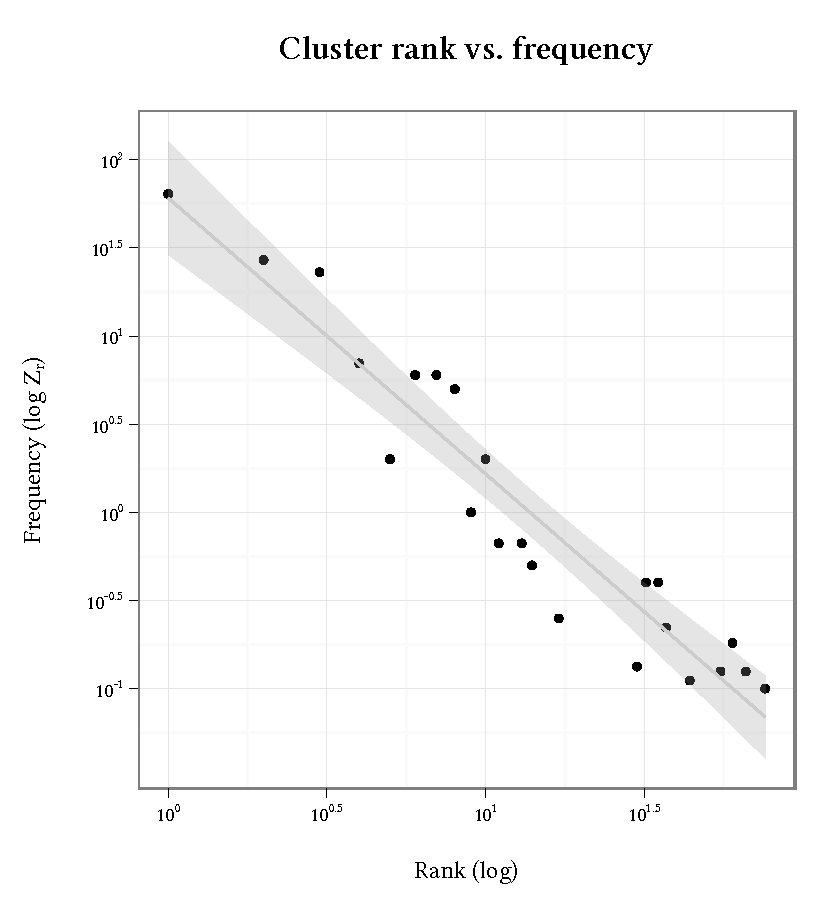
\includegraphics{cluster.pdf}
\caption{Syllable contact clusters, themselves composed of Zipfian medial codas and medial onsets, also exhibit a Zipfian distribution.}
\label{clus}
\end{figure}

That clusters (and the codas and onsets that make them up conforms to Zipf's law is not itself a deep observation. Zipfian distributions are characteristic of both syntactic rules \citep{Yang2009}, but also word \citep{Teahan1998,Ha2002,Baroni2009} and phoneme \citep{Daland2011a} n-grams, and tokens in non-linguistic symbol systems \citep{Chomsky1958,Sproat2010} or randomly-generated texts \citep{Miller1957,Li1992}. The import of this statistical property for the study of cluster phonotactics is that it makes it difficult, on statistical grounds alone, to determine which unobserved events are excluded, and which are accidentally missing. 

\citet{Good1953} puts forth a simple theory of just how frequent unobserved events might be. He proposes to estimate $\hat{p}_0$, the probability of all unseen events, as the ratio of events which occur just once $n_1$, to the number of observations, $\sum N$. This quantity is known as the Good-Turing estimate, since it was originally developed by Alan Turing for codebreaking during the second World War.

\begin{unlabeledexample}
$\displaystyle \hat{p}_0 = \frac{n_1}{\sum N}$ 
\end{unlabeledexample}

\noindent In the CELEX data, $65$ clusters occur only once, and there are 873 clusters in all, so $\hat{p}_0 = 0.074$. One way to interpret this quantity is with respect to a ``replication''. If it were possible to generate a new corpus of syllable contact clusters, approximately 7\% of cluster tokens will be ones that were not attested in the previous sample, i.e., they accidentally failed to be sampled. This is a not-inconsiderable quantity. 

Unfortunately, the Good-Turing estimate does not provide a way to determine which unattested clusters might be found in a replication. But I have already proposed that the null hypothesis of generative phonology, combined with the principle of Stampean occultation, provides a way out of this conundrum. Unattested clusters like *[m.kl] are structurally excluded (since such a cluster is occulted by \textsc{Coda Nasal Place Assimilation}), whereas *[s.l] is probably an accidental gap.

\subsubsection{Sampling simulation}

As a final investigation into this data, I consider the statistical properties of a randomly generated novel ``lexicon''. The simulated lexicon is generated by  generating a distribution of clusters, by repeatedly applying the following procedure.

\begin{example}[Simulation procedure]
\begin{tabular}{l l}
a. & Sample a medial coda according to the observed probabilities  \\
b. & Sample a medial onset according to the observed probabilities \\
c. & Apply the SPE rules to the resulting cluster                  \\
\end{tabular}
\end{example}

\noindent This is a simulation version of the model proposed by \citet{Pierrehumbert1994} and \citet{Coleman1997}, but also takes occulting phonology into account. 

While this procedure can be repeated indefinitely 
%(using the CELEX data, listed in Appendix \ref{A}), 
consideration of a single characteristic run of the simulation should suffice. The saturation rate of the simulated sample (18.2\%) is very close to the real sample (18.8\%). The slope of the log-rank/log-frequency relationship for the simulated data ($\alpha = -0.557$) is also very close to the observed slope for the CELEX data ($\alpha = -0.588$). And, as shown in Figure \ref{sim}, the two distributions are nearly indistinguishable. 

\begin{figure}
\centering
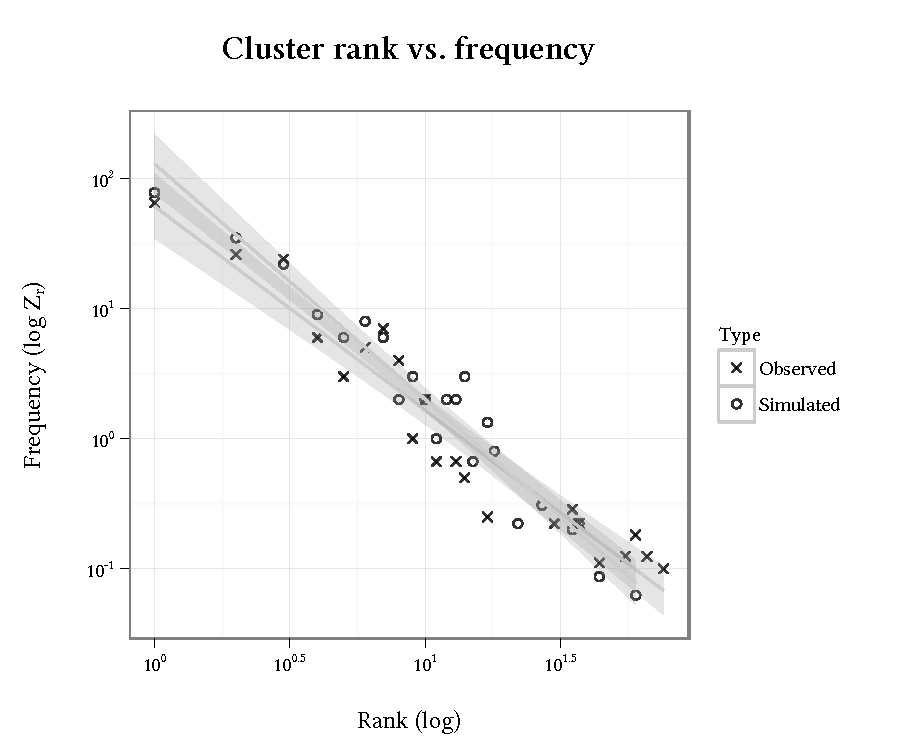
\includegraphics{sim.pdf}
\caption{A comparison of the observed lexical frequencies of English syllable contact clusters to an ``English lexicon'' simulated by combining.}
\label{sim}
\end{figure}

It is important to note that the results of this simulation should not be construed as an endorsement of a revised version of the \citet{Pierrehumbert1994} and \citet{Coleman1997} model which also incorporates occultation. In fact, as was shown above, the independent frequencies of coda and onset are very poor predictors of what clusters will be attested even when occultation is taken into account, and the set of attested clusters only partially overlaps those produced by the simulation. I propose that this is because the lexicon is not only finite, but far smaller than the combinatoric possibilities provided by phoneme sequences, making accidental gaps unavoidable. That these gaps will be arbitary from the perspective of phonology is nothing more than a corrolary of the principle of \emph{l'arbitraire du signe}. 

It is quite possible that phonology (and, perhaps, static phonotactics) acts as a filter on what URs are learned, but a cluster might be overrepresented or underrepresented for reasons that are quite external to phonology, e.g., language contact or historical change. Similarly, the factors that cause a /n/ to be a common word-medial coda in English may be independent of the propensity of that coda to combine with medial onset, assuming the resulting cluster is phonologically licit. The import of this simulation is somewhat more subtle; it simply shows free combination of codas and onsets according to their independent probabilities, constrained only by occultation, would produce the same sparse distribution of clusters that was used to argue for static phonotactics.

%\citet{Evert2004}
%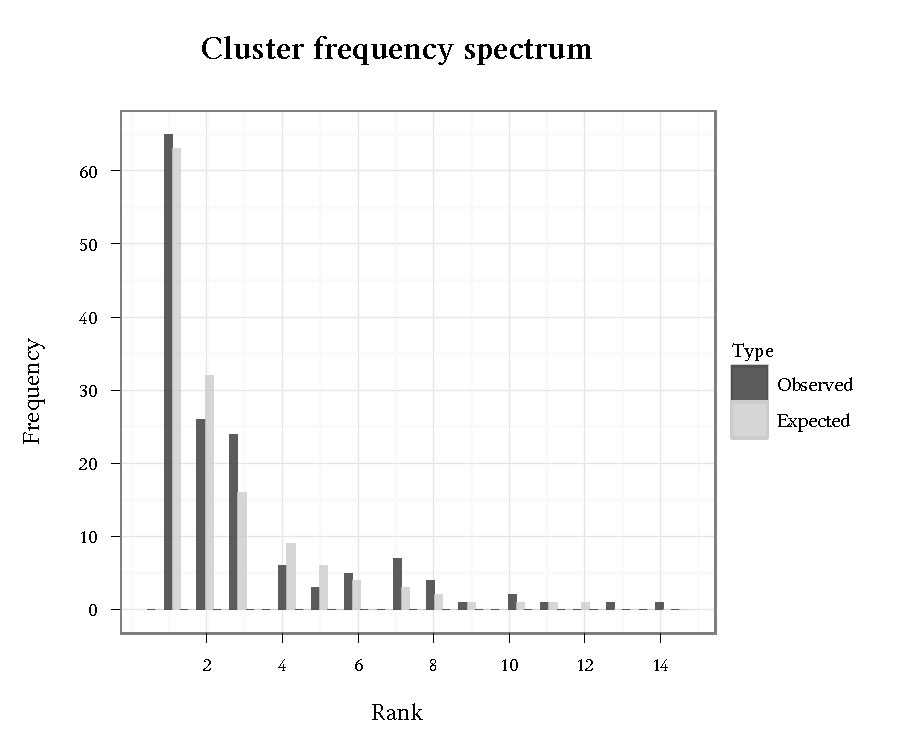
\includegraphics{zipf.pdf}

\section{Conclusions}

\citet{Borowsky1989} on peripherality.

productive \citet{Duanmu2008}

The above is a stark reminder.


A reasonable objection to the arguments presented in this chapter is to view the results as little more than an indictment of the results of \citealt{Pierrehumbert1994}.

However, the fact that state-of-the-art models are not capable of providing large improvements to the predictive accuracy indicates


 do not have a statistically significant effect on the shape of the English lexicon, but that experiments might turn up evidence that speakers have internalized 


shown to be aware of static constraints if they reached statistical significance. 



 statistically reliable static constraints could be identified 

The of


Regarding the historical developments,

\citet{Martin2007}

On the other hand, patterns created by sound change are not guaranteed to persist over time. One example of non-persistence is discussed by \citet{Iverson2005}. Around 1100 CE, Old English \emph{sk} became [ʃ]. This sound change introduced no alternations. Since long vowels were not found before tautosyllabic syllable clusters at this time, there were no \emph{V\lm sk\#} words when the change was actuated, and \emph{V\lm sh\#} continues to be rare in Modern English. What \citeauthor{Iverson2005} observe, however, is that there is nothing apparently peripheral about words like \emph{leash} or \emph{whoosh}, and loanwords and coinages have readily filled the gap.

\citet[][140]{Frisch2004} suggest that the strong tendency for the first and second consonants of the Arabic root to be non-identical is the ``a diachronic result of a processing constraint that disfavors repetition.'' Unfortunately, there is no evidence that this pattern is diachronic other than in the sense that it appears to be inherited from the proto-language: there is simply no Proto-Semitic verb roots with identical first and second consonants \citep[][178]{Greenberg1950}. In other Semitic languages, the inherited patern has experienced considerable erosion. 

\begin{example}[Tigrinya roots with identical first and second consonants \citep{Buckley1990a}]
\begin{tabular}{l l l l}
a. & lʌlʌw     & `scorch'                   & (\textless{} Ge'ez \emph{lʌwlʌw} `inflame')     \\
   & mʌmʌy     & `winnow'                   & (\textless{} Ge'ez \emph{mʌymʌy} `distinguish') \\
   & mʌmʌt     & `pick out loot'            \\
b. & s’ʌs’ʌw   & `finish off a drink'       & (cf. \emph{s’ʌws’ʌw} `gulp down')           \\
   & t’ʌt’ʌf   & `prune tree'               & (cf. \emph{t’ʌft’ʌf} `smear wall with mud') \\
c. & kʷakʷkʷʌr & `waste away, be emaciated' & (cf. \emph{kʷarkʷʌr} `interrogate')         \\
   & kakʷkʷɨʕ  & `clean wax from ears'      & (cf. \emph{kaʕkʷɨʕ} `start to form pods')   \\
\end{tabular}
\end{example}

Similar exceptions are found in 
%Amharic (\citealp[][?]{Broselow1984}, \citealp[][?]{McCarthy1985}) and 
Hebrew \citep[][29]{Bat-El2005}.

The next two chapters return to the question of synchrony, addressing the relationship between statistical patterns in the lexicon and speakers' behaviors when presented with underrepresented sequences.

accidental gaps
\citet[][419f.]{Hayes2008a}
